\clearpage
\section{Cracking Pattern caused by Pure DEF Expansion}

%*******10********20********30********40********50********60********70********80
\subsection{Single DEF Expansion Simulation}

In this section, the relationship between DEF intensified part range and concrete behavior during DEF expansion is simulated. The expanse is generated at the location of interfaces between paste element, to introduce the DEF expansion, as introduced in chapter 2.

For DEF expansion is highly related to the curing temperature concrete experienced, it is reasonable to considerate the inner part of the concrete structure should present more severe expansion comparing with outer part, due to its higher maximum experienced temperature during steam curing.

For surrounding part of the model, cases of non-expansion and gradually decreasing expansion are considered.

In this section, 100x100x100mm model is using. For comparison, 3 different cases are simulated, which are intensified 50x50x50mm at the center of the model, intensified 75x75x75mm at the center of the model, and intensified all part of the model (100x100x100mm).

\begin{figure}[ht]
\centering
    %*******
    \begin{subfigure}{.33\textwidth}
      \centering
      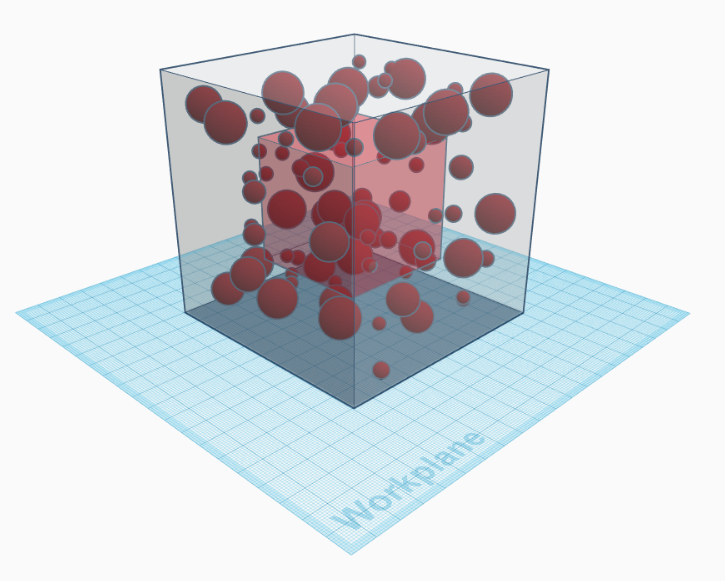
\includegraphics[width=.8\linewidth]{Files/DEF_X/X0_3d.png}
      \caption{Intensified  \\ 50x50x50mm Case}
    \end{subfigure}%
    %*******
    \begin{subfigure}{.33\textwidth}
      \centering
      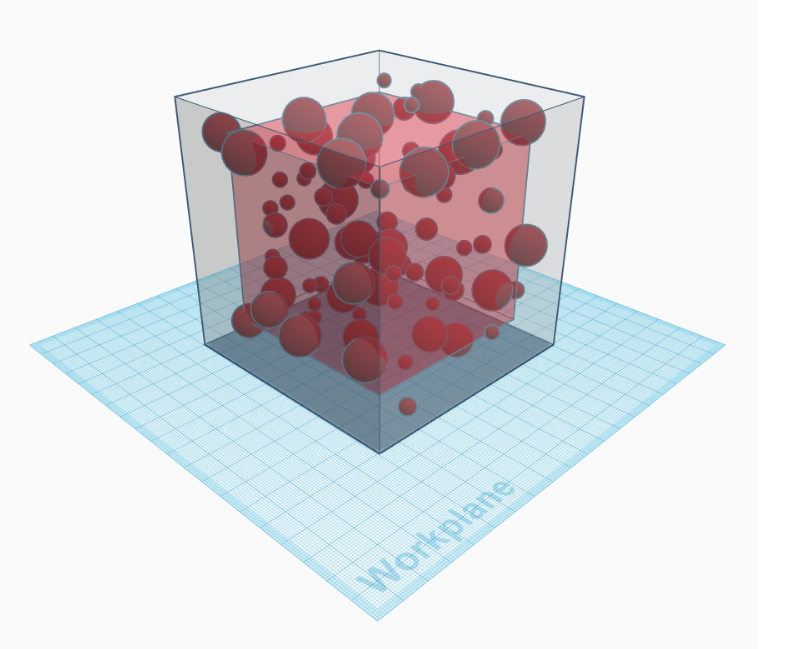
\includegraphics[width=.8\linewidth]{Files/DEF_X/X-5_3d.png}
      \caption{Intensified  \\ 75x75x75mm Case}
    \end{subfigure}%
    %*******
    \begin{subfigure}{.33\textwidth}
      \centering
      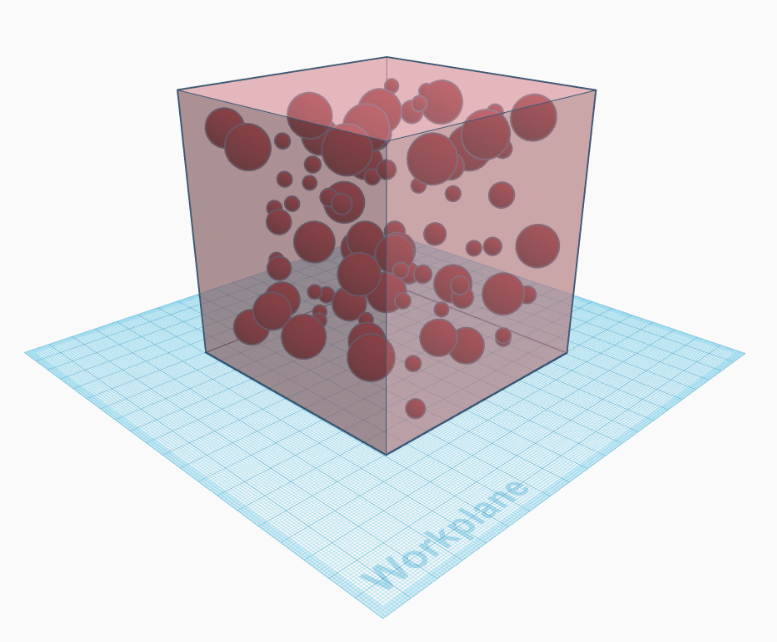
\includegraphics[width=.8\linewidth]{Files/DEF_X/X-1_3d.png}
      \caption{Intensified  \\ 100x100x100mm Case}
    \end{subfigure}
    %*******
    %*******
    \begin{subfigure}{.33\textwidth}
      \centering
      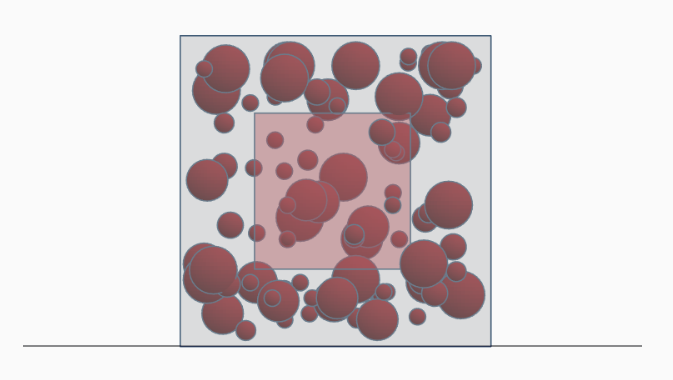
\includegraphics[width=.8\linewidth]{Files/DEF_X/X0_3ds.png}
      \caption{Intensified  \\ 50x50x50mm Case\\ Cross Section}
    \end{subfigure}%
    %*******
    \begin{subfigure}{.33\textwidth}
      \centering
      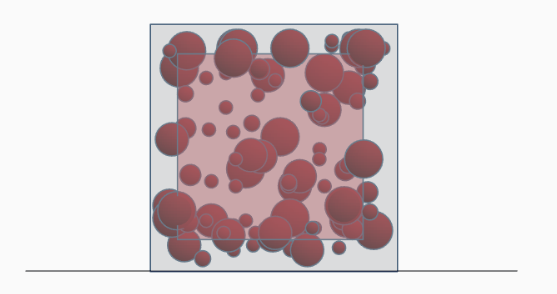
\includegraphics[width=.8\linewidth]{Files/DEF_X/X-5_3ds.png}
      \caption{Intensified \\  75x75x75mm Case \\ Cross Section}
    \end{subfigure}%
    %*******
    \begin{subfigure}{.33\textwidth}
      \centering
      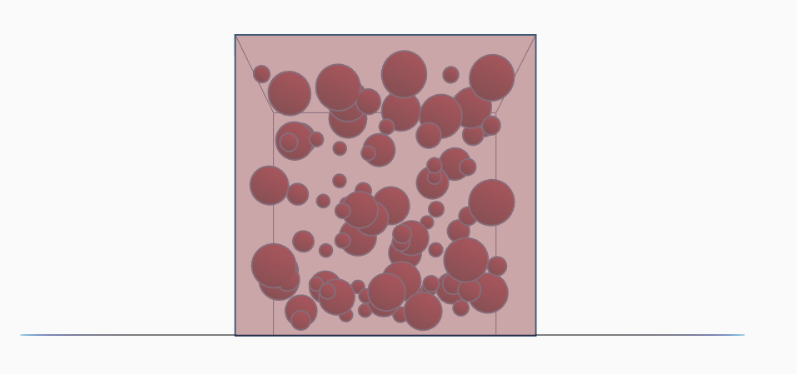
\includegraphics[width=.9\linewidth]{Files/DEF_X/X-1_3ds.png}
      \caption{Intensified  \\ 100x100x100mm Case\\ Cross Section}
    \end{subfigure}
    %*******
  \caption{DEF intensified part range}
  \label{fig:DEF_X}
\end{figure}

This single example case showing here as an example has been choosing here use the model in the dimension of 100x100x100mm, with 30\% aggregate, of which center 50x50x50mm have intensified DEF reactive, and the expanding giving to the model gradually decrease to 0 in the surrounded part.

\begin{figure}[ht]
\centering
    %*******
    \begin{subfigure}{.33\textwidth}
      \centering
      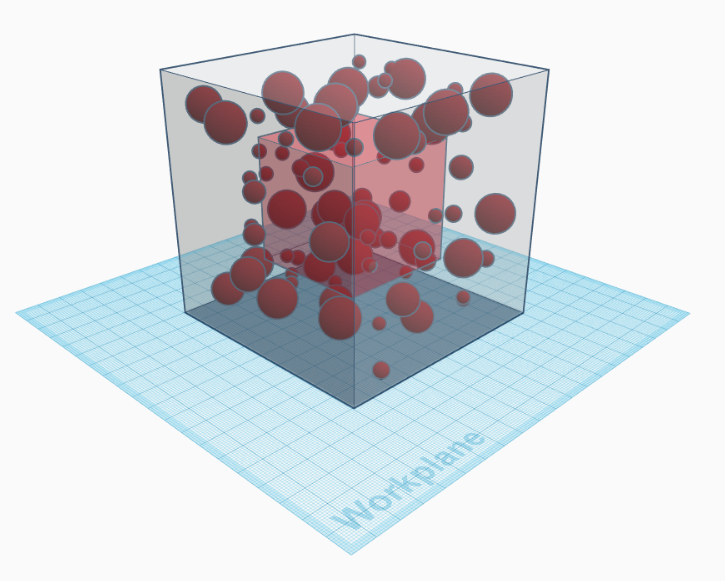
\includegraphics[width=.8\linewidth]{Files/DEF_X/X0_3d.png}
      \caption{Intensified \\ 50x50x50mm Case}
    \end{subfigure}%

    \begin{subfigure}{.33\textwidth}
      \centering
      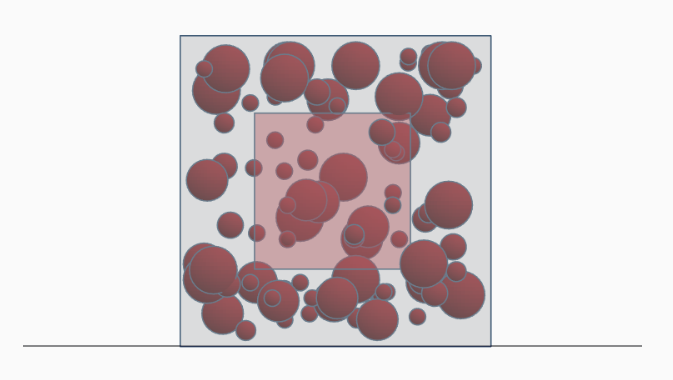
\includegraphics[width=.8\linewidth]{Files/DEF_X/X0_3ds.png}
      \caption{Intensified \\  50x50x50mm Case\\ Cross Section}
    \end{subfigure}%
    %*******

  \caption{50x50x50mm DEF intensified part range}
  \label{fig:DEF_X0}
\end{figure}


%TODO: X0 illustration

  \begin{figure}[ht]
  \centering
  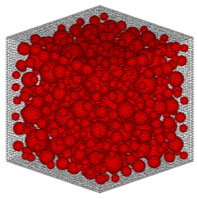
\includegraphics[width=.3\linewidth]{Files/Aggregate/A30.png}
    \caption{30\% Coarse Aggregate}
    \label{fig:A30_model}
  \end{figure}

Table. Aggregate consistent(if we have it)

To simulate DEF expansion, an initial strain of 0.0004mm is given in intensified DEF expanding area in each step, and the initial strain gradually decrease to 0 for surrounded parts, for totally 20 steps expansion.

%TODO: X0 D0.0004 Initial Strain

  \begin{table}[ht]
  \centering
  \begin{tabular}{ ||p{3cm}|p{3cm}||p{3cm}|p{3cm}|| }
  \hline
   Step &  Expansion & Step & Expansion \\
   \hline\hline
    1 & 0.000235  & 11 & 0.003061 \\
    2 & 0.000506  & 12 & 0.003355 \\
    3 & 0.000776  & 13 & 0.003650 \\
    4 & 0.001051  & 14 & 0.003949 \\
    5 & 0.001329  & 15 & 0.004249 \\
    6 & 0.001615  & 16 & 0.004555 \\
    7 & 0.001900  & 17 & 0.004865 \\
    8 & 0.002188  & 18 & 0.005175 \\
    9 & 0.002478  & 19 & 0.005487 \\
    10 & 0.002768 & 20  & 0.005795 \\
    \hline
    \end{tabular}
  \caption{Expansion in Each Step for A30 Case 3}
  \label{table:A30X0C_3_EXP}
  \end{table}

  \begin{figure}[ht!]
  \centering
  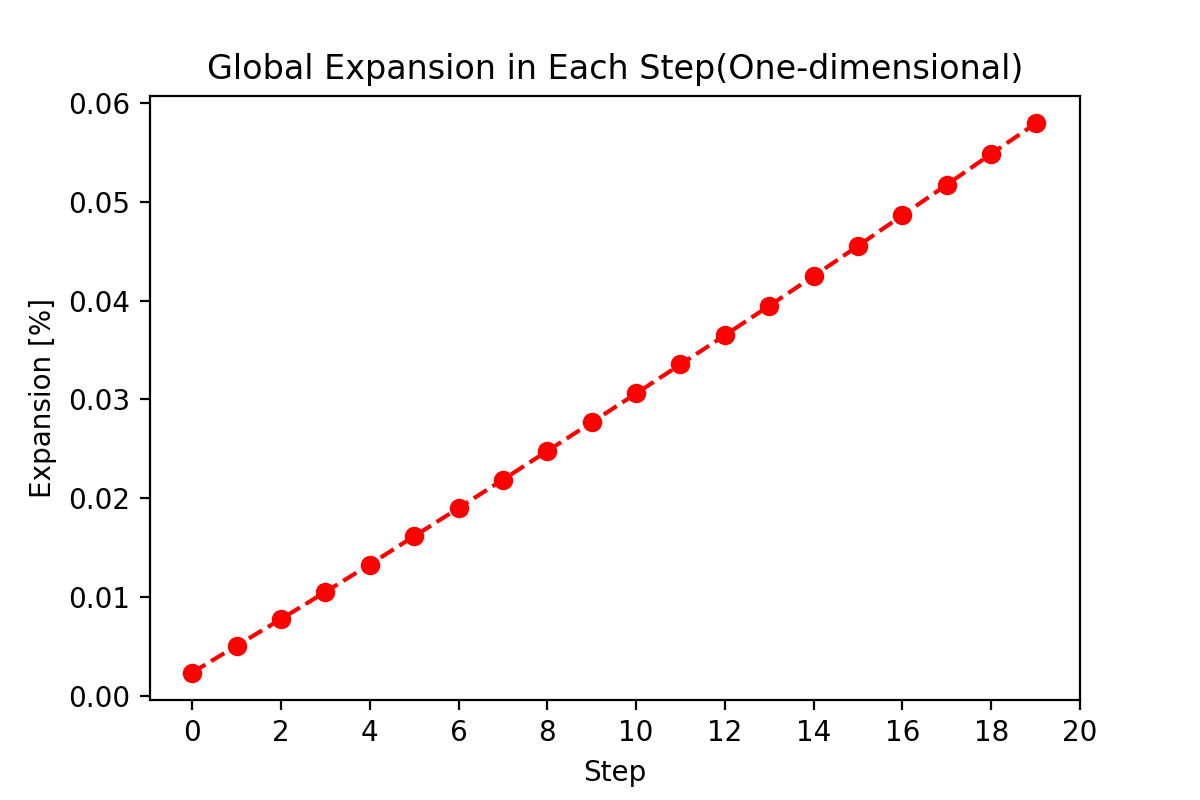
\includegraphics[width=.8\linewidth]{Files/exp_plot/DEFA30X0C_3_exp.png}
    \caption{Global Expansion vs. Step}
    \label{fig:DEFA30X0C_3_exp}
  \end{figure}

With the increasing of initial strain giving, the global expansion also gradually increasing. After 20 steps of DEF expansion, the model here reached 0.5795\% expansion(one-dimensionally). Characteristic DEF map cracking pattern can be seen on the surface of the expanded concrete modelin Figure \ref{fig:DEF_A30X0C_3_3D}.

In Figure \ref{fig:DEF_A30X0C_3_crack}, the inner distribution of cracked interface with width greater than 0.03mm is presented. It can be seen that the cracks are located with very clear patterns, concentrated in the inner part of the model. This inner cracking distribution pattern is very different with the cases ASR expansion.

  \begin{figure}[ht!]
  \centering
      %*******
      \begin{subfigure}{.5\textwidth}
        \centering
        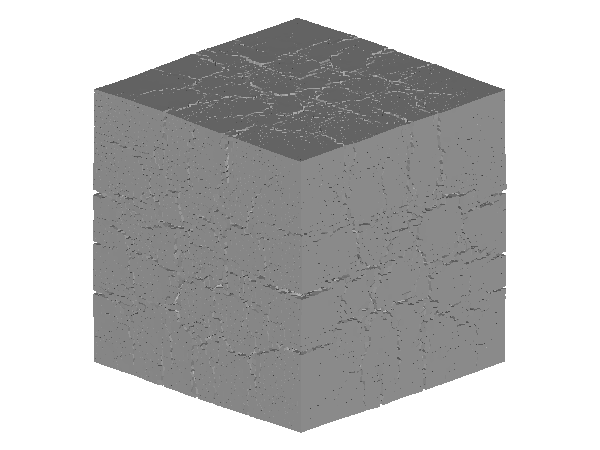
\includegraphics[width=.8\linewidth]{Files/exp_3D/DEF/A30X0C_3_3d.png}
      \end{subfigure}%
      \begin{subfigure}{.5\textwidth}
        \centering
        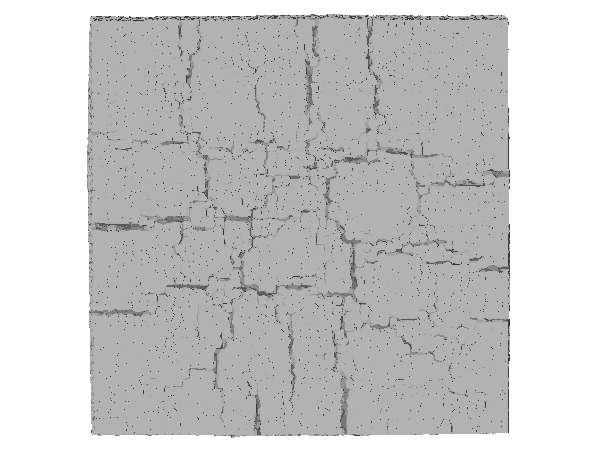
\includegraphics[width=.8\linewidth]{Files/exp_3D/DEF/A30X0C_3_3ds.png}
        \end{subfigure}
        %*******
    \caption{3D Surface Cracks, 0.4223\% Expansion (Deformation x 10)}
    \label{fig:DEF_A30X0C_3_3D}
  \end{figure}

  \begin{figure}[ht]
  \centering
      %*******
      \begin{subfigure}{.5\textwidth}
        \centering
        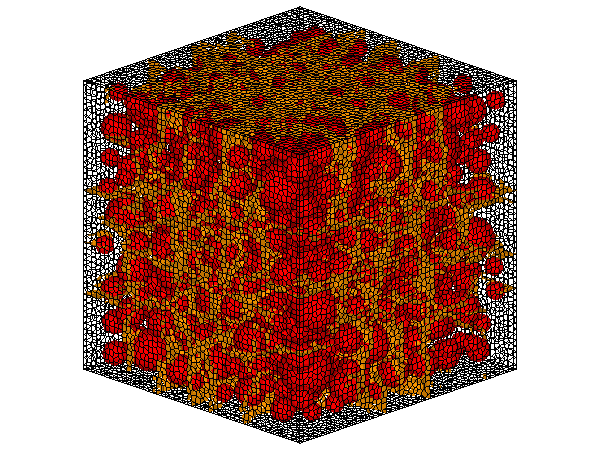
\includegraphics[width=.8\linewidth]{Files/exp_3D/DEF/A30X0C_3_c.png}
      \end{subfigure}%
    \label{fig:DEF_A30X0C_3_crack}
    \caption{3D Inner Cracks, 0.4223\% Expansion}
  \end{figure}

% DEF_A30_X0C_3

  \begin{figure}[ht!]
  \centering
      %*******
      \begin{subfigure}{.25\textwidth}
        \centering
        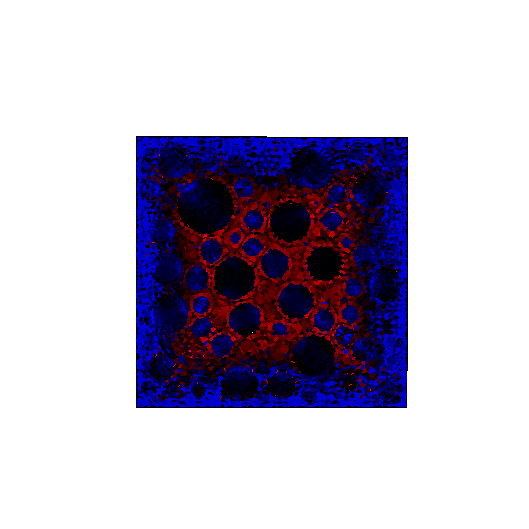
\includegraphics[width=1.0\linewidth]{Files/A30X0C_3_IS/DEP50-STEP(001).png}
      \caption{Step 1}
      \end{subfigure}%
      %*******
      \begin{subfigure}{.25\textwidth}
        \centering
        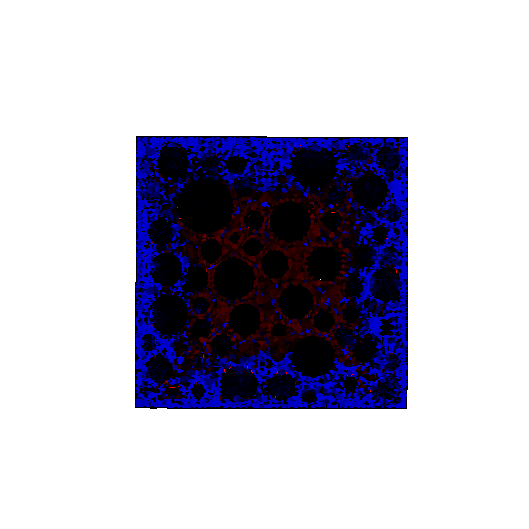
\includegraphics[width=1.0\linewidth]{Files/A30X0C_3_IS/DEP50-STEP(002).png}
      \caption{Step 2}
      \end{subfigure}%
      %*******
      \begin{subfigure}{.25\textwidth}
        \centering
        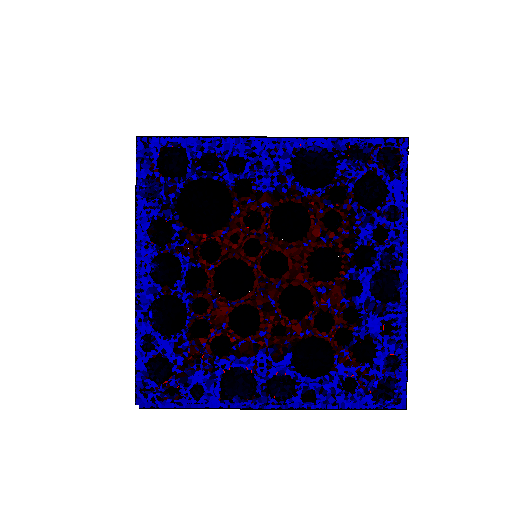
\includegraphics[width=1.0\linewidth]{Files/A30X0C_3_IS/DEP50-STEP(003).png}
      \caption{Step 3}
      \end{subfigure}%
      %*******
      \begin{subfigure}{.25\textwidth}
        \centering
        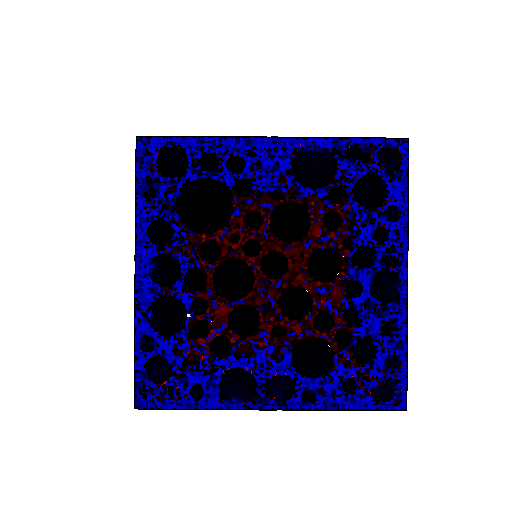
\includegraphics[width=1.0\linewidth]{Files/A30X0C_3_IS/DEP50-STEP(004).png}
      \caption{Step 4}
      \end{subfigure}

      %*******
      %*******
      \begin{subfigure}{.25\textwidth}
        \centering
        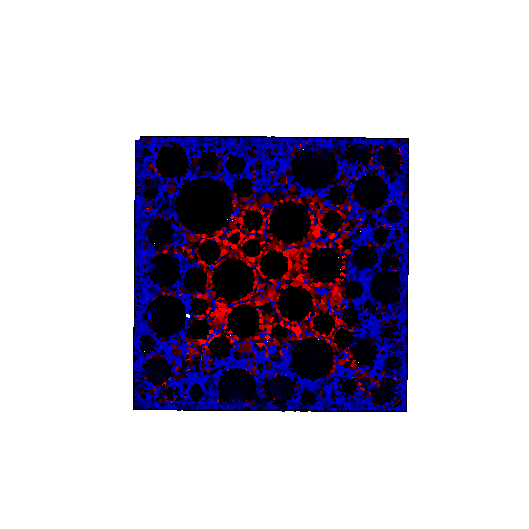
\includegraphics[width=1.0\linewidth]{Files/A30X0C_3_IS/DEP50-STEP(005).png}
      \caption{Step 5}
      \end{subfigure}%
      %*******
      \begin{subfigure}{.25\textwidth}
        \centering
        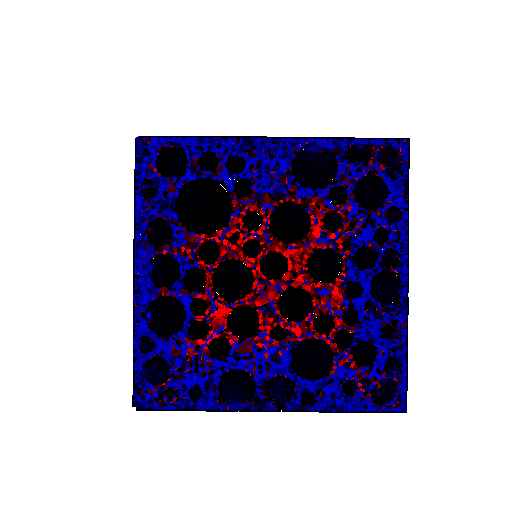
\includegraphics[width=1.0\linewidth]{Files/A30X0C_3_IS/DEP50-STEP(006).png}
      \caption{Step 6}
      \end{subfigure}%
      %*******
      \begin{subfigure}{.25\textwidth}
        \centering
        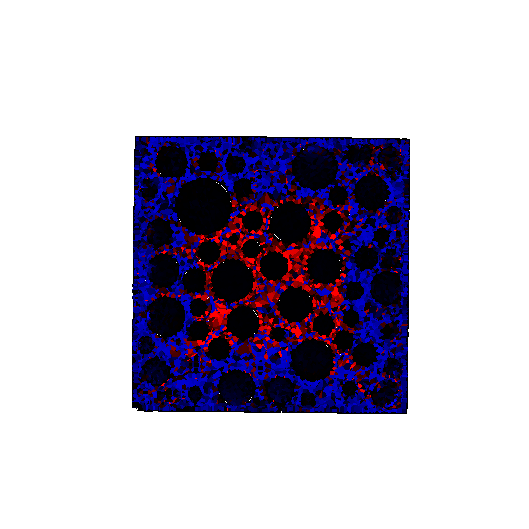
\includegraphics[width=1.0\linewidth]{Files/A30X0C_3_IS/DEP50-STEP(007).png}
      \caption{Step 7}
      \end{subfigure}%
      %*******
      \begin{subfigure}{.25\textwidth}
        \centering
        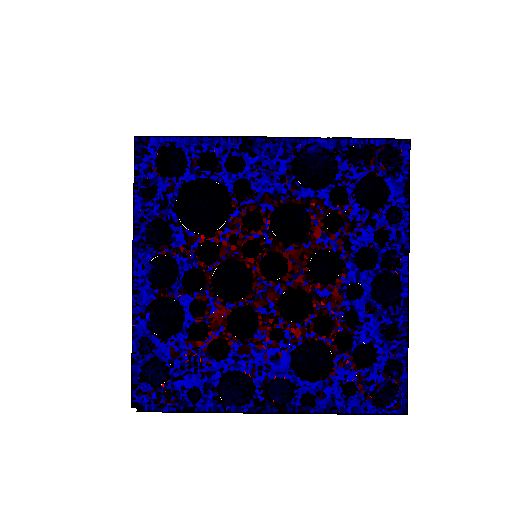
\includegraphics[width=1.0\linewidth]{Files/A30X0C_3_IS/DEP50-STEP(008).png}
      \caption{Step 4}
      \end{subfigure}

      %*******
      %*******
      \begin{subfigure}{.25\textwidth}
        \centering
        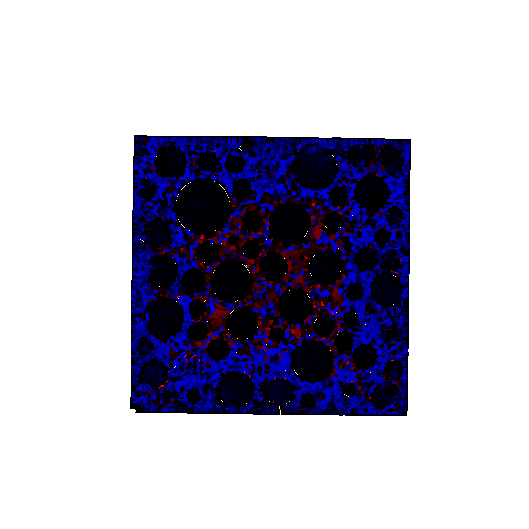
\includegraphics[width=1.0\linewidth]{Files/A30X0C_3_IS/DEP50-STEP(009).png}
      \caption{Step 9}
      \end{subfigure}%
      %*******
      \begin{subfigure}{.25\textwidth}
        \centering
        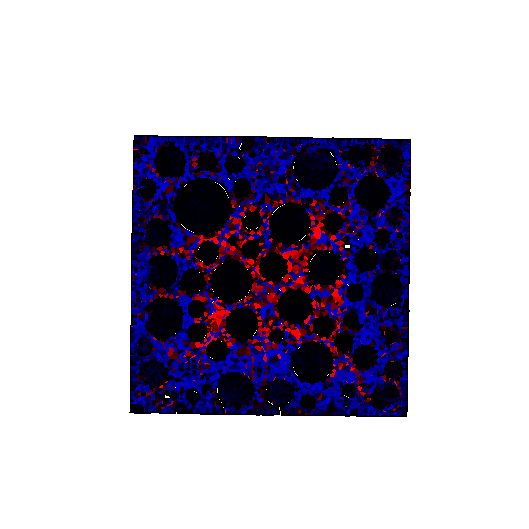
\includegraphics[width=1.0\linewidth]{Files/A30X0C_3_IS/DEP50-STEP(010).png}
      \caption{Step 10}
      \end{subfigure}%
      %*******
      \begin{subfigure}{.25\textwidth}
        \centering
        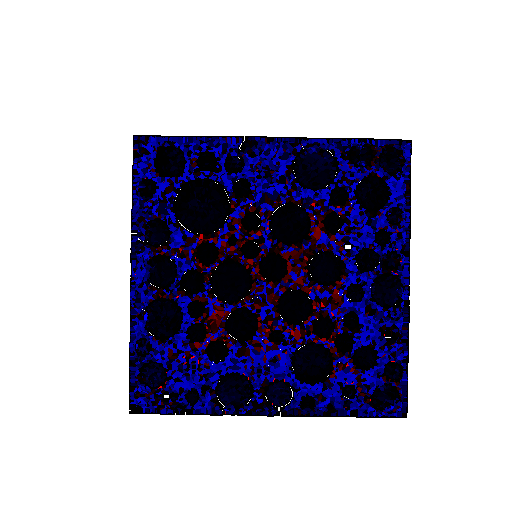
\includegraphics[width=1.0\linewidth]{Files/A30X0C_3_IS/DEP50-STEP(011).png}
      \caption{Step 11}
      \end{subfigure}%
      %*******
      \begin{subfigure}{.25\textwidth}
        \centering
        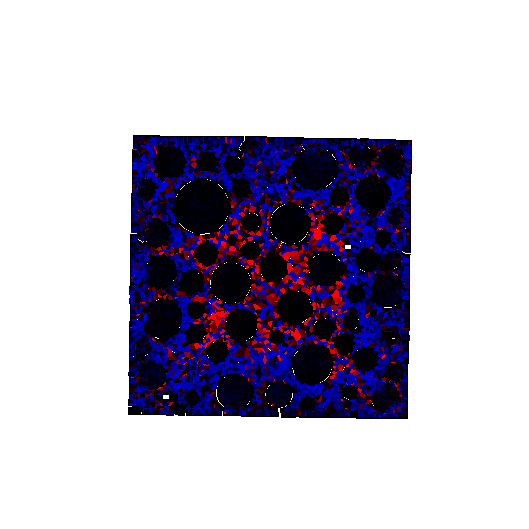
\includegraphics[width=1.0\linewidth]{Files/A30X0C_3_IS/DEP50-STEP(012).png}
      \caption{Step 12}
      \end{subfigure}

      %*******
      %*******
      \begin{subfigure}{.25\textwidth}
        \centering
        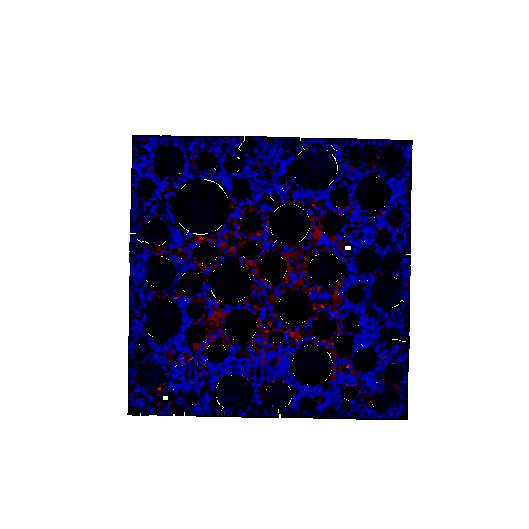
\includegraphics[width=1.0\linewidth]{Files/A30X0C_3_IS/DEP50-STEP(013).png}
      \caption{Step 13}
      \end{subfigure}%
      %*******
      \begin{subfigure}{.25\textwidth}
        \centering
        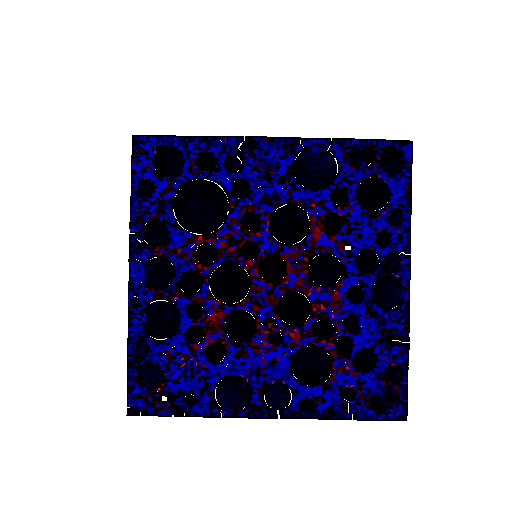
\includegraphics[width=1.0\linewidth]{Files/A30X0C_3_IS/DEP50-STEP(014).png}
      \caption{Step 14}
      \end{subfigure}%
      %*******
      \begin{subfigure}{.25\textwidth}
        \centering
        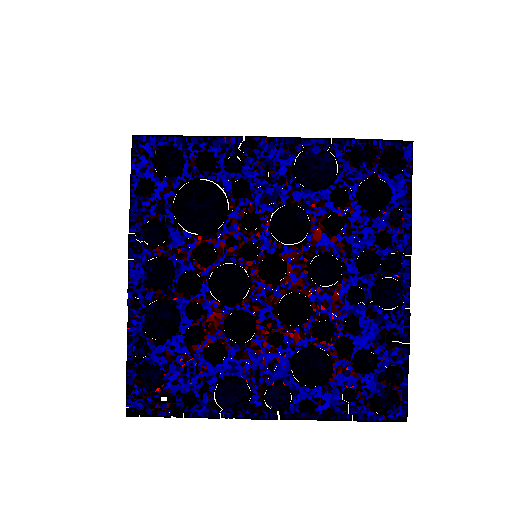
\includegraphics[width=1.0\linewidth]{Files/A30X0C_3_IS/DEP50-STEP(015).png}
      \caption{Step 15}
      \end{subfigure}%
      %*******
      \begin{subfigure}{.25\textwidth}
        \centering
        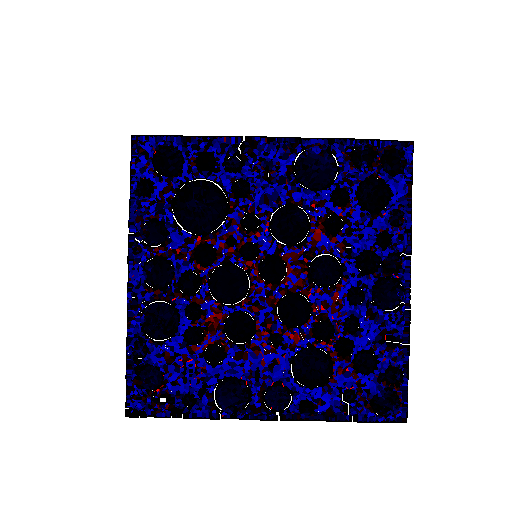
\includegraphics[width=1.0\linewidth]{Files/A30X0C_3_IS/DEP50-STEP(016).png}
      \caption{Step 16}
      \end{subfigure}

      %*******
      %*******
      \begin{subfigure}{.25\textwidth}
        \centering
        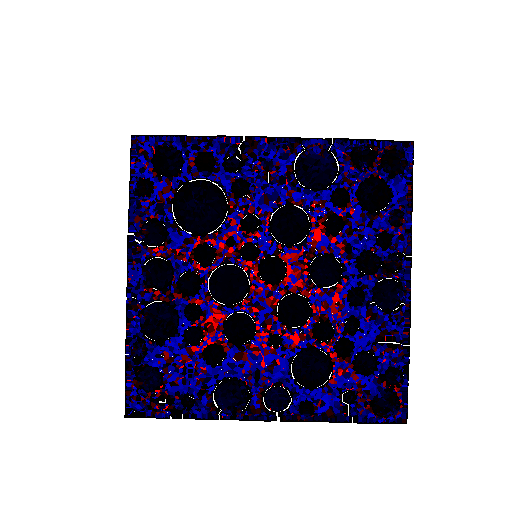
\includegraphics[width=1.0\linewidth]{Files/A30X0C_3_IS/DEP50-STEP(017).png}
      \caption{Step 17}
      \end{subfigure}%
      %*******
      \begin{subfigure}{.25\textwidth}
        \centering
        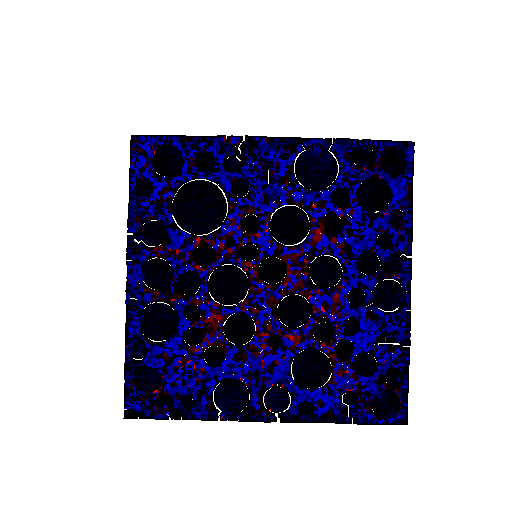
\includegraphics[width=1.0\linewidth]{Files/A30X0C_3_IS/DEP50-STEP(018).png}
      \caption{Step 18}
      \end{subfigure}%
      %*******
      \begin{subfigure}{.25\textwidth}
        \centering
        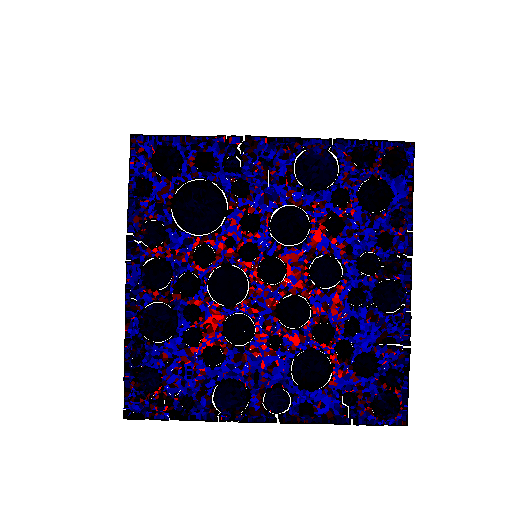
\includegraphics[width=1.0\linewidth]{Files/A30X0C_3_IS/DEP50-STEP(019).png}
      \caption{Step 19}
      \end{subfigure}%
      %*******
      \begin{subfigure}{.25\textwidth}
        \centering
        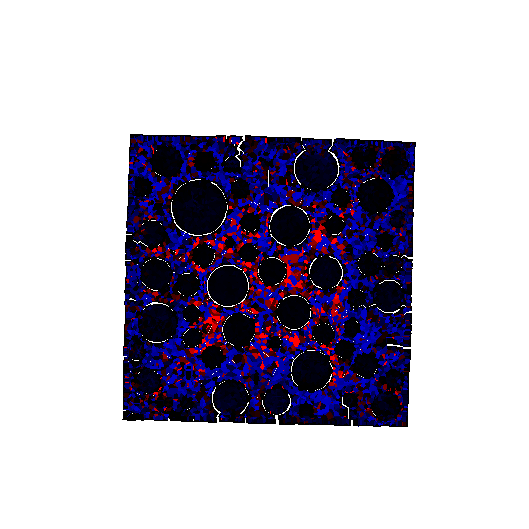
\includegraphics[width=1.0\linewidth]{Files/A30X0C_3_IS/DEP50-STEP(020).png}
      \caption{Step 20}
      \end{subfigure}

      \begin{subfigure}{0.8\textwidth}
  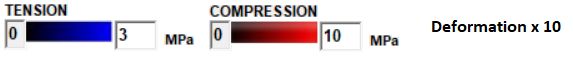
\includegraphics[width=0.8\linewidth]{Files/exp_3D/tagCS10.png}
\end{subfigure}%


  \caption{Internal Stress in Each Step for A30 X0C Case 3 (Deformation x 10)}
  \label{fig:DEF_A30X0C_3_IS}
  \end{figure}

As can be seen in Figure \ref{fig:DEF_A30X0C_3_IS} the compressive stress (in red color) first concentrated in the part where initial strain is intensified given, and from step 1 to 20, unbalanced force penetrated in the concrete model, crack generated gradually around the aggregate and the surrounding part of the model.

Same as previous in ASR expansion simulation,  cracked interfaces are summarised in different crack width scale, shown in Table \ref{table:A30X0C_3_Cracks}. The maximum crack width, in this case, is in range of 0.01-0.03mm, while most of the cracks still under 0.001mm. The number of cracked interfaces gradually decreases with the increase of crack width.

\begin{table}[!h]
\centering
\begin{tabular}{ |p{4cm}|p{5cm}| }
\hline
 Crack Width [mm] &  Total Cracked Interfaces \\
 \hline\hline

   0.00000 - 0.00005 & 367538 \\
   0.00005 - 0.00010 & 328471 \\
   0.00010 - 0.00020 & 294472 \\
   0.00020 - 0.00050 & 251035 \\
   0.00050 - 0.00100 & 186058 \\
   0.00100 - 0.00300 & 133854 \\
   0.00300 - 0.01000 & 57421 \\
   0.01000 - 0.03000 & 1736 \\
   0.03000 - 0.10000 & 0 \\
   0.1000+ & 0 \\

  \hline
  \end{tabular}
\caption{Expansion in Each Step for A30 X0C Case 3}
\label{table:A30X0C_3_Cracks}
\end{table}
